% !TeX root = ../main.tex
% 修改稿迁移版：自动编号，原文数据与待核事项保留。
\chapter{市场与竞争分析}
\section{市场现状}\label{sec:4.1}
智能体运行基础设施已经形成企业可采购的产品和服务。专业沙箱平台与大型云服务商共同参与市场：E2B 提供面向智能体的独立运行环境，AWS 提供 AgentCore 运行与工具服务，阿里云提供智能体运行和沙箱服务。PI OS 将在现有供给格局中，围绕国产环境适配、资源效率和企业交付建立差异化能力。

\NumberedPara{1}{企业智能体应用正在扩大，配套运行需求随之增加}
德勤《2026 年企业人工智能现状报告》基于对 24 个国家、3,235 名企业与技术负责人的调查显示，23\% 的受访企业已经至少中等程度地使用智能体，74\% 预计在未来两年内达到这一水平。其中，74\% 为受访者对未来两年的预期，23\% 为当前采用情况，两者之间的差距反映了企业扩大应用的意愿。

PI OS 优先面向已经使用智能体执行代码、处理文件和调用工具的企业。这类应用需要实际的任务执行环境，与沙箱产品的需求直接相关。项目计划从代码修复、功能开发等明确场景切入，围绕真实任务量验证客户需求。

\NumberedPara{2}{沙箱服务已形成收费模式，细分方向获得资本关注}
截至\textbf{2026 年 9 月 5 日}，E\textbf{2}B 的 Pro 套餐公开价格为\textbf{150 美元/\allowbreak{}月}，资源使用费用另计；套餐包含最多\textbf{100}个同时运行的沙箱，并允许付费增加并发额度。这表明沙箱服务已经形成按照使用规模、运行资源和服务等级收费的商业模式。

融资方面，E\textbf{2}B 于\textbf{2025 年 7 月}宣布完成\textbf{2,100 万美元}A 轮融资，累计融资达到\textbf{3,200 万美元}。该案例表明，智能体执行基础设施已受到专业投资机构关注。融资数据反映资本关注度，营业收入和盈利能力仍需通过经营数据验证。

PI OS 将围绕客户付费理由推进产品化，并在商业化授权明确后，通过部署适配、持续维护和服务支持建立收入来源。

\NumberedPara{3}{企业仍在增加投入，但成本正在影响应用规模}
麦肯锡于\textbf{2026 年 8 月}发布的全球调查覆盖\textbf{97 个国家}的\textbf{1,719 名受访者}。调查显示，约\textbf{20\%}的受访者表示，包含模型调用费用在内的 AI 运营成本已经限制了所在企业的 AI 使用；与此同时，\textbf{60\%}预计企业将在未来一年增加 AI 投入。两项结果共同说明，企业在继续增加 AI 投入的同时，更加重视新增投入带来的业务价值。

这种成本关注也体现在现有产品设计中。AWS AgentCore 已采用按实际 CPU 消耗和会话内存占用计费的方式，在没有 CPU 消耗的等待期间不收取 CPU 费用。由此可见，提高资源使用效率已经成为服务商参与竞争的一个方向。

PI OS 的商业价值应以客户实际账本衡量：在相同任务质量与服务要求下，减少资源投入或让已有服务器完成更多任务。沙箱优化对应整体 AI 成本中的执行环境部分，项目将单独核算其资源和运维改善幅度。

\NumberedPara{4}{企业需求存在差异，为适配与交付服务提供切入点}
德勤报告显示，\textbf{85\%}的受访企业预计需要定制智能体，以适应自身业务需求。调查结果说明，企业应用需要结合业务流程、工具组合和运行环境进行适配。

阿里云等厂商已提供自定义镜像、代码执行、浏览器操作和存储接入等能力，适配与集成已经成为市场基础能力。PI OS 将把国产操作系统适配、有限资源下的任务承载能力和交付服务作为可验证的差异化方向。

企业采用、公开收费和资本参与等信号表明，智能体执行基础设施已经进入商业化阶段。PI OS 将通过客户试点验证付费转化，当前重点是识别具有明确任务规模、部署要求和采购预算的客户。

\section{市场前景}\label{sec:4.2}
智能体运行基础软件的市场需求正在从开发工具延伸到企业业务中的持续运行服务。从近期研究与公开案例看，企业希望让智能体承担更完整的工作流程；而一旦走向规模化应用，部署效率、运行成本和可靠性就会成为更高门槛。PI OS 的近期市场机会，集中在已经开展试点并计划扩大任务规模的企业------这类客户既需要高效的执行环境，也需要专业的交付服务。

\subsection{市场趋势和驱动因素}\label{sec:4.2.1}
\NumberedPara{1}{智能体从单项工具走向业务流程，运行服务需求有望持续扩大}
德勤于\textbf{2026 年 8 月 12 日}发布的调查显示，\textbf{74\%}的受访管理者预计，未来四年内，所在企业近一半的业务流程将围绕智能体重新设计；但目前只有\textbf{15\%}的受访企业已经规模化采用跨职能、多智能体协同。这项调查覆盖美国五个行业的\textbf{501}名管理者，参与企业均已至少开展智能体试点，数据反映了已有应用基础企业的扩展预期。

企业后续需求包括多任务稳定运行、现有业务系统连接和持续增长的工作量管理。PI OS 可优先面向已经开展试点、正在扩大使用范围的客户，通过任务承载能力和交付质量争取采购机会。

\NumberedPara{2}{AI 基础设施投入增长，为配套运行软件提供发展空间}
Gartner 于\textbf{2026 年 8 月 10 日}发布预测，全球 AI 优化型基础设施即服务（IaaS）支出将在\textbf{2026}年达到\textbf{422.76}亿美元，同比增长\textbf{96.4\%}；\textbf{2027}年预计进一步达到\textbf{661.43}亿美元。预测数据显示，支撑 AI 实际运行的基础设施仍处于较快投入阶段。

\FloatBarrier
\begingroup\linespread{1}\selectfont
\setcounter{table}{0}
\begin{longtable}{@{}>{\raggedright\arraybackslash}p{\dimexpr 0.24997\linewidth-1.4998\tabcolsep\relax}>{\raggedright\arraybackslash}p{\dimexpr 0.24997\linewidth-1.4998\tabcolsep\relax}>{\raggedright\arraybackslash}p{\dimexpr 0.24997\linewidth-1.4998\tabcolsep\relax}>{\raggedright\arraybackslash}p{\dimexpr 0.25008\linewidth-1.5005\tabcolsep\relax}@{}}
\caption{全球 AI 优化型 IaaS 支出及预测}\label{tab:4-1}\\
\hline
\rowcolor{WordTableHeader} \TableHeaderText{年份} & \TableHeaderText{支出规模（亿美元）} & \TableHeaderText{同比增速} & \TableHeaderText{数据性质} \\ \hline
\endfirsthead
\multicolumn{4}{c}{\fontsize{9}{12}\selectfont 表 4-1（续）}\\
\hline
\rowcolor{WordTableHeader} \TableHeaderText{年份} & \TableHeaderText{支出规模（亿美元）} & \TableHeaderText{同比增速} & \TableHeaderText{数据性质} \\ \hline
\endhead
\hline\endfoot\hline\endlastfoot
\rowcolor{WordTableStripe} 
2025 年 & 215.29 & 180.0\% & 报告列示的基期值 \\ \hline
2026 年 & 422.76 & 96.4\% & 机构预测 \\ \hline
\rowcolor{WordTableStripe} 
2027 年 & 661.43 & 56.5\% & 机构预测 \\ \hline
\end{longtable}\endgroup
上述规模覆盖模型训练、推理等基础设施支出，统计口径大于智能体沙箱市场。其对 PI OS 的参考价值在于：企业持续投入 AI 基础设施，将带动资源效率优化、部署维护和配套软件服务需求。

\NumberedPara{3}{投资关注点将更加重视使用成本与实际回报}
IDC 于\textbf{2026 年 8 月 28 日}发布的研究解读指出，相关调查中，\textbf{67\%}的企业在过去一年内的智能体支出超过预算\textbf{10\%}以上。该统计覆盖智能体整体支出，其中沙箱对应执行环境部分的成本，数据反映了规模化应用中的成本管理压力。

据此，PI OS 的商业化重点应落在能够核算的客户收益上：在相同任务质量和响应要求下，是否能够减少资源投入、延缓扩容，或提高已有服务器的任务完成量。后续报价与续约应建立在实际效果和服务质量上。

\subsection{智能体运行服务的应用领域广泛}\label{sec:4.2.2}
以下案例来自公开资料，用于说明行业应用方向；PI OS 的实际客户和交付能力以项目合同与测试记录为准。

\textbf{1}）软件研发与自动化测试

代码修复、功能开发和测试执行与 PI OS 的企业命题直接对应，是项目最适合优先进入的场景。E\textbf{2}B 于\textbf{2026 年 7 月}公布的 Devin Outposts 集成方案，支持开发任务在企业可控制的云环境中执行，并访问私有代码仓库和内部服务，体现了研发智能体对执行环境与企业系统接入的需求。

PI OS 可围绕企业研发团队和代码智能体平台，验证并发任务承载、任务完成质量及部署维护成本，形成首批可复制的交付案例。

\textbf{2}）数据分析与研究报告生成

数据分析智能体需要执行程序、处理文件并生成可使用的结果。E\textbf{2}B 于\textbf{2026 年 5 月}披露的 Genspark 案例，展示了沙箱在数据分析、研究和报告生成等多步骤任务中的应用。

数据分析场景可作为 PI OS 在代码任务之外的延伸方向，面向数据分析平台和企业内部研究工具提供运行支持，重点验证文件处理、较长任务运行和多用户使用的稳定性。

\textbf{3}）企业办公与业务流程自动化

人力资源、销售支持和文档处理等工作，往往需要连接多个系统并执行重复操作。E\textbf{2}B 于\textbf{2026 年 2 月}披露，Gumloop 已持续使用其代码执行服务两年多，应用覆盖智能体工具调用、自定义流程和系统集成。

这类应用需要持续的环境维护、版本适配和故障支持，可形成部署后的年度服务需求。PI OS 可在基础产品稳定后，与业务应用开发商合作进入此类市场。

\textbf{4}）金融与保险业务辅助

金融保险领域存在模型计算、表格处理和业务材料准备等执行需求。E\textbf{2}B 于\textbf{2026 年 8 月 5 日}披露，Effective AI 利用沙箱支持保险产品相关工作，月用户会话超过\textbf{1}万次。该数字来自厂商公开案例，项目评估时将结合独立客户数据复核。

金融保险领域对数据隔离、权限和过程记录提出较高要求。PI OS 将在完成相应验证后，通过行业合作伙伴进入辅助分析与材料处理场景，创业初期的服务范围限定在辅助性任务。

\textbf{5}）模型评测与科研实验

模型评测需要反复执行大量任务，并保证不同实验之间互不影响。E2B 于 2026 年 9 月 3 日披露，Paper Instruments 使用其沙箱运行数千个并发实验任务，每个任务保留独立的文件与执行状态。

批量评测工作负载与高密部署具有较强关联。PI OS 可面向模型研发团队和科研机构，探索批量评测服务，重点验证单位资源能够完成的实验数量，以及实验环境的一致性。

\textbf{6}）工业工程与制造业研发

智能体的应用也在向专业工程领域延伸。西门子于\textbf{2026 年 4 月 20 日}发布 Eigen Engineering Agent，并披露该产品此前已在\textbf{19 个国家}、超过\textbf{100}家客户中试点，支持工业自动化工程任务。

对 PI OS 而言，潜在切入点是工程代码、测试脚本和研发辅助任务的执行环境。该领域可作为中长期拓展方向，需要结合专业软件适配和行业合作逐步推进。

PI OS 的市场拓展分为三个阶段：首阶段聚焦代码任务，第二阶段扩展数据分析与批量评测，第三阶段通过合作进入专业行业。项目收入将以客户试点收益、付费转化和可复制交付为依据。

\section{目标市场}\label{sec:4.3}
PI OS 面向需要批量运行人工智能智能体的企业和科研机构，提供智能体执行环境及配套部署服务。智能体执行环境为 AI 提供代码运行、程序测试和数据处理所需的隔离空间。PI OS 在满足任务质量与安全要求的前提下，提高客户现有服务器的任务承载能力，降低智能体规模化应用的运行成本。

麦肯锡于 2026 年 8 月发布的全球调查显示，在年营收超过 10 亿美元的大型企业受访者中，报告所在企业正在规模化部署智能体的比例由上年的 27\% 上升至 40\%；较小企业的对应比例为 22\%。智能体规模化应用较集中的职能包括信息技术、知识管理和软件工程。该调查覆盖 97 个国家的 1,719 名受访者，用于反映全球样本趋势；中国市场情况仍需结合本地客户验证。

基于上述需求分布，PI OS 将首先进入软件研发和智能体开发场景，优先服务已经拥有实际任务、部署预算和内部技术团队的客户，再逐步拓展科研平台及行业解决方案市场。

\subsection{PI OS 具有以下重要特点}\label{sec:4.3.1}
\begin{enumerate}
\item 面向智能体实际工作的运行需求
\end{enumerate}
PI OS 聚焦智能体程序执行、工具调用和文件处理，为客户现有大模型和业务系统补充执行环境。客户可以在保留现有系统架构的基础上评估和接入 PI OS。

该定位聚焦客户已有工作流程，通过真实任务检验产品价值，并缩小客户的系统改造范围。

\begin{enumerate}
\item 以现有设备的使用效率创造价值
\end{enumerate}
PI OS 围绕运行时扁平化、动态资源卸载和智能内存共享开展研发，商业目标是减少运行环境中的重复占用和无效等待，提高同等设备条件下的任务承载能力。

客户价值体现在减少任务排队、延缓服务器扩容和降低合格任务的综合成本。上述收益将通过客户实际环境中的对照测试确认。

\begin{enumerate}
\item 面向国产运行环境与企业部署需求
\end{enumerate}
项目以华为命题指定的国产运行环境为适配方向，规划提供客户自有服务器或云环境中的部署、调试和维护服务，支持客户结合自身的系统配置与管理要求使用产品。

企业对智能体的需求具有明显的业务差异。德勤 2026 年 1 月发布的调查显示，85\% 的受访企业预计会根据自身业务需求定制智能体。该调查于 2025 年 8---9 月开展，覆盖 24 个国家的 3,235 名企业与信息技术负责人。调查结果支持项目对企业适配服务的关注，沙箱软件采购需求将通过客户访谈和试点进一步确认。

\subsection{PI OS 现阶段目标市场}\label{sec:4.3.2}
PI OS 的市场进入顺序为企业场景、科研验证和渠道合作。

\FloatBarrier
\begingroup\linespread{1}\selectfont
\setcounter{table}{1}
\begin{longtable}{@{}>{\raggedright\arraybackslash}p{\dimexpr 0.23878\linewidth-1.4327\tabcolsep\relax}>{\raggedright\arraybackslash}p{\dimexpr 0.32832\linewidth-1.9699\tabcolsep\relax}>{\raggedright\arraybackslash}p{\dimexpr 0.20893\linewidth-1.2536\tabcolsep\relax}>{\raggedright\arraybackslash}p{\dimexpr 0.22397\linewidth-1.3438\tabcolsep\relax}@{}}
\caption{PI OS 目标客户与市场进入顺序}\label{tab:4-2}\\
\hline
\rowcolor{WordTableHeader} \TableHeaderText{目标客户} & \TableHeaderText{主要应用场景} & \TableHeaderText{主要采购决策方} & \TableHeaderText{市场进入安排} \\ \hline
\endfirsthead
\multicolumn{4}{c}{\fontsize{9}{12}\selectfont 表 4-2（续）}\\
\hline
\rowcolor{WordTableHeader} \TableHeaderText{目标客户} & \TableHeaderText{主要应用场景} & \TableHeaderText{主要采购决策方} & \TableHeaderText{市场进入安排} \\ \hline
\endhead
\hline\endfoot\hline\endlastfoot
\rowcolor{WordTableStripe} 
智能体应用开发企业、AI 编程平台 & 代码修复、功能开发、自动测试等任务的批量执行 & 技术负责人、研发平台负责人 & 优先争取付费验证与部署项目 \\ \hline
企业内部研发中心 & 在现有服务器上运行内部研发智能体 & 研发管理部门、信息化部门 & 以具体部门或项目试点切入 \\ \hline
\rowcolor{WordTableStripe} 
高校实验室、研究所及模型评测团队 & 智能体实验、代码能力评测、重复任务验证 & 课题负责人、科研平台管理部门 & 形成可复核案例，按项目预算采购 \\ \hline
云服务商、软件厂商及系统集成商 & 将执行引擎纳入自身产品或行业方案 & 产品部门、解决方案部门 & 在产品标准化后拓展合作 \\ \hline
\end{longtable}\endgroup
\NumberedPara{1}{企业软件研发与智能体平台市场}
这类客户直接面对智能体任务的运行费用、任务完成速度和服务稳定性，是项目优先争取的商业客户。项目计划从代码修复、自动测试等边界清晰的任务切入，用客户已有系统与 PI OS 方案完成同一批任务，比较任务完成情况、设备占用和维护投入。

对于已经存在运行压力的客户，采购理由可以具体落实到“是否需要增加服务器”“任务是否能够按时完成”，有利于形成明确的预算依据。

\NumberedPara{2}{高校、研究所和企业研究院市场}
科研客户适合开展新方案验证、重复实验和性能评测。PI OS 计划提供研究环境部署、任务运行支持和实验数据整理服务，帮助科研团队减少环境配置及重复运维工作。

目标客户包括拥有真实计算任务和项目经费的实验室、研究团队及公共平台。科研合作、免费试用与实际采购收入分别统计。

\NumberedPara{3}{云服务与行业解决方案市场}
完成标准化交付后，PI OS 计划向云服务商和系统集成商提供运行引擎集成、环境适配及维护支持。合作方负责上层应用和客户服务，PI OS 聚焦智能体执行环节，并借助已有销售渠道扩大覆盖范围。

现阶段市场测算以可触达客户、试点转化率和实际合同金额为基础，并按照 PI OS 的可交付范围核算服务市场。

\section{商业模式}\label{sec:4.4}
\subsection{商业模式概述}\label{sec:4.4.1}
PI OS 采用“部署适配服务 + 年度软件与维护服务”的企业级商业模式，相关业务将在成果商用授权和产品验收完成后启动。

项目初期优先利用客户已有服务器和云资源开展交付，由客户承担自身计算资源费用，PI OS 收取需求分析、安装部署、系统适配和持续维护等费用。对于具备合法商业许可条件的产品版本，再提供年度软件订阅。

该模式将初期资金集中用于产品完善和客户交付，并控制自建大规模算力设施的资金投入。标准化程度提高后，业务将由一次性项目交付逐步转向可重复部署的软件产品和持续服务。

客户转化流程包括：

需求确认 → 小范围验证 → 验收采购 → 正式部署 → 年度续费与扩容。

其中，小范围验证重点回答三个问题：能否完成客户任务、综合成本是否具有改善空间、接入与维护投入是否可以接受。

\subsection{客户细分}\label{sec:4.4.2}
\begin{enumerate}
\item 智能体应用开发企业
\end{enumerate}
这类客户将智能体能力作为对外产品或服务，需要稳定承接用户任务。其主要关注运行费用、任务完成速度，以及业务增长后能否平稳扩容。

PI OS 提供执行环境接入、部署调优和持续支持，帮助客户将研发资源更多投入上层产品。

\begin{enumerate}
\item 企业内部平台建设部门
\end{enumerate}
这类客户为企业内部的多个团队建设统一研发或智能体平台，更关注系统兼容性、运行可控性和长期服务保障。

PI OS 按照客户已有设备、网络和运维流程开展部署，并提供配置文档、故障处理方式和升级安排。

\begin{enumerate}
\item 科研与评测机构
\end{enumerate}
科研与评测机构重视环境可复现、任务批量执行和实验结果可追溯。项目按照课题或平台建设需求提供部署与技术支持，商业转化以合同金额和持续采购为主要指标。

\begin{enumerate}
\item 产品集成与渠道客户
\end{enumerate}
这类客户购买的是能够嵌入自身方案的产品能力及支持服务。合作重点包括版本兼容、交付责任、维护边界及终端客户支持机制，收入方式通过具体合作协议确定。

\subsection{合作伙伴和资源}\label{sec:4.4.3}
项目的现有研究基础与华为、天津大学开展的“Agentic 运行时分层状态卸载与共享技术合作项目”相关。已有合作材料能够支持企业需求来源和研究方向的真实性，为项目开展命题适配、方案完善和工程验证提供基础。

商业化过程中，项目将重点整合三类资源：

\begin{enumerate}
\item 研究与工程资源：将已有代码、测试方法和技术积累转化为可安装、可验证、可维护的产品。
\item 场景与验证资源：争取具有真实任务的企业和科研机构参与试点，形成经客户确认的交付案例。
\item 生态与渠道资源：在产品成熟后，与国产操作系统生态、云服务商和系统集成商探索适配及联合交付。
\end{enumerate}
现有科研合作主体与未来创业经营主体分别管理。合同项下成果的使用、许可及对外展示须遵守既有权属和保密约定；科研合作材料用于说明技术来源，客户采购和营业收入以商业合同为准。

\subsection{可持续发展和扩展性}\label{sec:4.4.4}
\NumberedPara{1}{将重复交付内容产品化}
项目将安装配置、环境检查、常见任务接入和故障诊断整理为标准工具与文档，减少每个客户的重复开发工作。通用需求进入标准版本，特殊需求单独评估和收费，以控制定制项目对研发资源的占用。

\NumberedPara{2}{通过持续服务形成续费收入}
智能体框架、业务任务和客户环境会持续变化。项目围绕版本升级、兼容性维护、运行诊断和容量规划提供年度服务，使收入来源由一次性交付逐步延伸至持续维护。

\NumberedPara{3}{从单点试用扩展至多团队部署}
市场拓展从一个可验证场景开始，客户确认效果后，再扩展至其他项目组、服务器或业务部门。客户内部扩展能够降低重复获客成本，交付范围根据试点稳定程度逐步扩大。

\NumberedPara{4}{以经营质量衡量增长}
项目将持续跟踪付费验证转化率、交付周期、单客户服务投入、续费率和毛利情况。增长质量由客户数量、同类项目复制效率和单位研发人力产出共同衡量。

\subsection{收费模式}\label{sec:4.4.5}
PI OS 分阶段提供以下收费方式：

\NumberedPara{1}{验证与部署服务}
针对需求明确的客户，按约定任务开展验证，交付测试结果、适配说明和部署方案。涉及客户专有系统改造的工作另行报价，免费验证的任务范围和周期在协议中明确。

\NumberedPara{2}{企业年度订阅}
在相关成果获得商业使用授权后，按产品版本、管理规模和服务等级提供年度订阅。客户使用自有计算资源，软件订阅费用与服务器、云资源及大模型调用费用分别列示。

\NumberedPara{3}{专项适配与维护}
对于特殊系统、专用工具和非标准业务流程，按项目工作范围收费。年度合同之外的重大改造，通过新增服务订单确定。

\NumberedPara{4}{后续托管服务}
计量、稳定性和单位成本完成验证后，项目将评估托管式服务，并采用资源包或按量计费。当前阶段聚焦部署、适配和年度订阅服务。

\subsection{收费规则}\label{sec:4.4.6}
PI OS 的统一销售价格将在付费试点后确定。当前计费规则以交付成本、客户规模和试点结果为依据。

\FloatBarrier
\begingroup\linespread{1}\selectfont
\setcounter{table}{2}
\begin{longtable}{@{}>{\raggedright\arraybackslash}p{\dimexpr 0.12504\linewidth-0.7503\tabcolsep\relax}>{\raggedright\arraybackslash}p{\dimexpr 0.21425\linewidth-1.2855\tabcolsep\relax}>{\raggedright\arraybackslash}p{\dimexpr 0.33929\linewidth-2.0357\tabcolsep\relax}>{\raggedright\arraybackslash}p{\dimexpr 0.32142\linewidth-1.9285\tabcolsep\relax}@{}}
\caption{PI OS 拟定收费规则}\label{tab:4-3}\\
\hline
\rowcolor{WordTableHeader} \TableHeaderText{收费项目} & \TableHeaderText{计费单位} & \TableHeaderText{主要交付内容} & \TableHeaderText{费用边界} \\ \hline
\endfirsthead
\multicolumn{4}{c}{\fontsize{9}{12}\selectfont 表 4-3（续）}\\
\hline
\rowcolor{WordTableHeader} \TableHeaderText{收费项目} & \TableHeaderText{计费单位} & \TableHeaderText{主要交付内容} & \TableHeaderText{费用边界} \\ \hline
\endhead
\hline\endfoot\hline\endlastfoot
\rowcolor{WordTableStripe} 
场景验证服务 & 项目 & 需求确认、基线测试、方案验证、结果报告 & 事先明确任务范围、周期与验收条件 \\ \hline
部署与系统适配 & 项目 & 安装配置、接口适配、上线支持、使用培训 & 超出约定范围的新增开发单独报价 \\ \hline
\rowcolor{WordTableStripe} 
企业软件订阅 & 年度基础费 + 约定管理规模 & 已获商业授权的软件版本及约定功能 & 管理规模按服务器节点等明确口径约定 \\ \hline
运维与升级服务 & 年度 & 故障支持、版本升级、兼容性维护 & 已包含在订阅中的服务不重复收费 \\ \hline
\rowcolor{WordTableStripe} 
托管运行服务 & 资源包或实际用量 & 运行环境及配套服务 & 后续推出，分别列明计算、存储等计费项 \\ \hline
\end{longtable}\endgroup
定价将同时考虑交付成本和客户获得的价值。客户价值通过同等任务质量要求下的综合成本比较确认，成本范围包括计算资源、软件服务、部署摊销、运维以及失败重试等相关投入，各项性能提升按照其实际影响范围计入成本测算。

项目也将提供可核对的用量与服务记录，明确免费验证范围、订阅期限、扩容方式及超额处理规则，降低客户对后续费用不确定性的顾虑。

\section{竞争分析}\label{sec:4.5}
\subsection{世界竞争环境分析}\label{sec:4.5.1}
智能体执行基础设施已经出现专业沙箱厂商与大型云平台共同参与的竞争格局。专业厂商主要围绕开发者接入和执行环境提供产品，大型云平台则将执行能力与模型、身份管理及运行管理等服务组合交付。

E2B 已提供云沙箱和客户自有环境部署选项；Daytona 的虚拟机沙箱支持保留内存状态的暂停与恢复；AWS AgentCore 则提供智能体运行环境及配套工具服务。上述能力已经成为智能体执行基础设施的常见配置，竞争差异将更多体现在资源效率、适配成本和交付质量。

PI OS 聚焦特定国产运行环境和真实任务负载，通过设备使用效率、部署适配和持续服务参与竞争。

本次调研未获得能够直接比较上述厂商沙箱业务市场份额的统一权威数据，因此竞争判断以公开产品能力、收费方式及交付条件为依据。

\subsection{国内竞争环境分析}\label{sec:4.5.2}
\NumberedPara{1}{国内云平台已进入智能体执行市场}
阿里云 FC 云沙箱已经公开不同运行状态下的计费规则；百度智能云 AX 提供代码执行、浏览器操作等智能体运行场景及配套管理能力。国内市场已经形成云平台产品供给，PI OS 将围绕自有部署、国产环境适配和专项运行优化建立差异化。

对已经使用相应云平台的客户而言，继续采购同一体系内的服务可能更便于接入和管理。PI OS 将优先寻找具有自有部署、指定国产环境或专项运行优化需求的客户。

\NumberedPara{2}{资源节约正在成为产品的共同竞争方向}
阿里云 FC 云沙箱的公开规则区分活跃、浅休眠和深休眠状态：浅休眠不收取 CPU 费用，深休眠不收取 CPU 和内存费用，但仍存在磁盘费用。AWS AgentCore 的运行环境也区分实际 CPU 消耗和内存消耗，等待期间仍可能产生内存费用。

PI OS 的竞争验证将比较同一批任务的综合投入、资源回收等待时间、任务失败率和维护成本。

\NumberedPara{3}{收费竞争已经具有公开参照}
截至 2026 年 9 月 5 日，部分厂商公布的计算资源单价如下。

\FloatBarrier
\begingroup\linespread{1}\selectfont
\setcounter{table}{3}
\begin{longtable}{@{}>{\raggedright\arraybackslash}p{\dimexpr 0.22894\linewidth-1.3737\tabcolsep\relax}>{\raggedright\arraybackslash}p{\dimexpr 0.16032\linewidth-0.9619\tabcolsep\relax}>{\raggedright\arraybackslash}p{\dimexpr 0.15274\linewidth-0.9164\tabcolsep\relax}>{\raggedright\arraybackslash}p{\dimexpr 0.45800\linewidth-2.7480\tabcolsep\relax}@{}}
\caption{相关产品公开计费参照}\label{tab:4-4}\\
\hline
\rowcolor{WordTableHeader} \TableHeaderText{产品} & \TableHeaderText{CPU 单价} & \TableHeaderText{内存单价} & \TableHeaderText{适用说明} \\ \hline
\endfirsthead
\multicolumn{4}{c}{\fontsize{9}{12}\selectfont 表 4-4（续）}\\
\hline
\rowcolor{WordTableHeader} \TableHeaderText{产品} & \TableHeaderText{CPU 单价} & \TableHeaderText{内存单价} & \TableHeaderText{适用说明} \\ \hline
\endhead
\hline\endfoot\hline\endlastfoot
\rowcolor{WordTableStripe} 
E2B Hobby/\allowbreak{}Pro & 0.0504 美元/\allowbreak{}vCPU·小时 & 0.0162 美元/\allowbreak{}GiB·小时 & 由官方秒单价换算；Pro 另有 150 美元/\allowbreak{}月套餐费。官方价格 \\ \hline
Daytona 通用计算 & 0.0504 美元/\allowbreak{}vCPU·小时 & 0.0162 美元/\allowbreak{}GiB·小时 & 按秒计费，存储等项目另计。官方价格 \\ \hline
\rowcolor{WordTableStripe} 
AWS AgentCore Runtime microVMs & 0.0895 美元/\allowbreak{}vCPU·小时 & 0.00945 美元/\allowbreak{}GB·小时 & CPU 按实际活跃消耗计费，内存按其官方规则计量。官方价格 \\ \hline
阿里云 FC 云沙箱 Std & 0.078 元/\allowbreak{}vCPU·小时 & 0.039 元/\allowbreak{}GiB·小时 & 中国内地邀测按量单价，不能视为面向全部客户正式开放的统一价格。官方价格 \\ \hline
\end{longtable}\endgroup
\par\noindent{\fontsize{9}{13}\selectfont\linespread{1}\selectfont 注：上述价格按各产品公开的币种、资源单位、运行状态和服务范围列示。完整价格比较还需核对存储、网络、模型调用、套餐及其他费用。}

以 E2B 公布的资源价格计算，配置为 2 vCPU、8 GiB 内存的运行环境，连续运行 1 小时的 CPU 与内存费用为：

2 \ensuremath{\times} 0.0504 + 8 \ensuremath{\times} 0.0162 = 0.2304 美元。

该算例包含 CPU 与内存资源费用。PI OS 的售价和利润测算还需纳入软件、部署、运维、网络、存储和模型调用等成本。计算依据：E2B 官方价格

公开价格为客户替代方案提供参照。PI OS 将以完整交付成本和客户任务成本参与竞争。

\NumberedPara{4}{市场拓展与服务能力同样重要}
国内竞争同时取决于产品性能、采购便利性、接入速度和持续支持。PI OS 将通过范围明确的付费验证、标准化部署和可追溯的服务记录建立客户信任，并逐步扩大应用范围。

\subsection{竞争对手}\label{sec:4.5.3}
PI OS 的竞争对象既包括商业沙箱平台，也包括客户基于现有技术自行建设的执行环境。各类方案的交付范围存在差异，比较时需要结合客户原有系统和采购需求。

\FloatBarrier
\begingroup\linespread{1}\selectfont
\setcounter{table}{4}
\begin{longtable}{@{}>{\raggedright\arraybackslash}p{\dimexpr 0.12900\linewidth-0.5160\tabcolsep\relax}>{\raggedright\arraybackslash}p{\dimexpr 0.48400\linewidth-1.9360\tabcolsep\relax}>{\raggedright\arraybackslash}p{\dimexpr 0.38700\linewidth-1.5480\tabcolsep\relax}@{}}
\caption{主要竞争方案与 PI OS 的进入方向}\label{tab:4-5}\\
\hline
\rowcolor{WordTableHeader} \TableHeaderText{竞争方案} & \TableHeaderText{已公开的产品特点} & \TableHeaderText{PI OS 拟争取的客户需求} \\ \hline
\endfirsthead
\multicolumn{3}{c}{\fontsize{9}{12}\selectfont 表 4-5（续）}\\
\hline
\rowcolor{WordTableHeader} \TableHeaderText{竞争方案} & \TableHeaderText{已公开的产品特点} & \TableHeaderText{PI OS 拟争取的客户需求} \\ \hline
\endhead
\hline\endfoot\hline\endlastfoot
\rowcolor{WordTableStripe} 
E2B & 提供智能体沙箱、自定义环境及自有环境部署选项。产品说明 & 指定国产环境中的适配、实际任务效率和本地交付支持 \\ \hline
Daytona & 提供沙箱运行环境，虚拟机类型支持保留内存状态的暂停与恢复。官方文档 & 对任务运行成本和部署条件有专项要求的场景 \\ \hline
\rowcolor{WordTableStripe} 
AWS AgentCore & 提供运行环境、代码执行等服务，采用相应资源计费规则。官方说明 & 希望围绕既有国产基础设施建设执行能力的客户 \\ \hline
阿里云 FC 云沙箱 & 区分运行与休眠状态，配套云端资源管理和计费。官方文档 & 自有部署及非标准环境中的适配与优化需求 \\ \hline
\rowcolor{WordTableStripe} 
百度智能云 AX & 覆盖代码执行、浏览器操作等场景及运行管理。产品说明 & 已有上层智能体应用、主要需要执行环节支持的客户 \\ \hline
企业自建方案 & 自行选择虚拟化、容器或开源组件，并承担集成和维护责任 & 希望减少自研维护投入、获得明确交付责任的客户 \\ \hline
\end{longtable}\endgroup
PI OS 当前已经完成相关代码开发，产品化交付、指定环境适配和商业验证将通过后续验收确认。项目现阶段的优势包括研究积累、命题匹配方向和专项优化能力，商业领先程度将在客户交付和付费验证后评估。

后续竞争验证将围绕四项指标展开：

\begin{enumerate}
\item 任务效果：同一批任务的成功完成情况是否保持稳定。
\item 综合成本：纳入资源、软件及运维投入后，是否具有采购价值。
\item 接入成本：客户需要改造多少现有系统，多久能够投入使用。
\item 持续保障：升级、故障恢复及问题处理能否形成稳定交付能力。
\end{enumerate}
\subsection{SWOT 分析}\label{sec:4.5.4}
\FloatBarrier
\begingroup\linespread{1}\selectfont
\setcounter{table}{5}
\begin{longtable}{@{}>{\raggedright\arraybackslash}p{\dimexpr 0.11685\linewidth-0.4674\tabcolsep\relax}>{\raggedright\arraybackslash}p{\dimexpr 0.41945\linewidth-1.6778\tabcolsep\relax}>{\raggedright\arraybackslash}p{\dimexpr 0.46370\linewidth-1.8548\tabcolsep\relax}@{}}
\caption{PI OS SWOT 分析}\label{tab:4-6}\\
\hline
\rowcolor{WordTableHeader} \TableHeaderText{类型} & \TableHeaderText{主要判断} & \TableHeaderText{对应策略} \\ \hline
\endfirsthead
\multicolumn{3}{c}{\fontsize{9}{12}\selectfont 表 4-6（续）}\\
\hline
\rowcolor{WordTableHeader} \TableHeaderText{类型} & \TableHeaderText{主要判断} & \TableHeaderText{对应策略} \\ \hline
\endhead
\hline\endfoot\hline\endlastfoot
\rowcolor{WordTableStripe} 
优势 S & 具有企业命题和相关研究基础；已有代码开发积累；聚焦智能体执行效率这一具体问题 & 以真实任务形成可复核成果，将研究积累转化为标准产品 \\ \hline
劣势 W & 商业产品成熟度、付费客户及续费表现尚待验证；早期交付可能依赖定制；成果商用存在授权前提 & 完成授权与产品验收，控制定制范围，优先形成少量高质量付费案例 \\ \hline
\rowcolor{WordTableStripe} 
机会 O & 企业正在扩大智能体应用，特定运行环境和业务流程存在适配需求 & 优先进入软件研发与评测场景，再扩展至平台和渠道合作 \\ \hline
威胁 T & 云平台与专业厂商持续完善产品，客户也可自建；功能竞争和价格竞争可能压缩利润空间 & 以任务成本、接入效率及持续服务建立差异，避免仅依赖单一功能竞争 \\ \hline
\end{longtable}\endgroup
SW 分析：优势与劣势

PI OS 聚焦明确的企业问题，已有代码和研究基础能够支持后续验证。商业化工作将这些积累转化为客户能够采购、部署和持续使用的产品。

项目当前重点包括明确成果使用权限、完善标准交付、获得付费验证，并形成真实的成本与续费数据。同类客户以较低新增投入完成部署后，技术积累将逐步转化为可持续的经营优势。

OT 分析：机会与威胁

智能体应用增长为执行基础设施带来需求，也吸引大型云平台和专业厂商持续投入。PI OS 的市场机会来自需求具体、价值可验证的细分领域，主要威胁包括产品同质化、客户沿用现有平台和客户自建方案。

项目从一个明确场景起步，在效果确认后复制到相似客户。长期竞争力由客户持续付费的运行效率、可靠交付和服务能力构成。

\section{企业调研与需求验证}\label{sec:4.6}
本节说明项目的一手调研过程与需求验证结果。第四章前五节主要依据公开报告与竞品资料判断市场方向，本节补充项目团队直接面向企业技术负责人、研发平台负责人和潜在采购决策方开展的访谈与需求确认，用于回答三个问题：客户当前用什么方案运行智能体、痛点出现在哪个环节、在什么条件下愿意为改进付费。调研记录按 I-01---I-10 编号归档，与表 1-1 的证据索引对应。

\par\noindent{\fontsize{9}{13}\selectfont\linespread{1}\selectfont 注：本节表格中标注“待填”的身份、时间与量化信息，应依据实际访谈记录（I-01---I-10）补齐后提交；未开展或未取得受访方同意的访谈内容不列入本表。本节为访谈整理的初步结论，代表受访对象的观点，不等同于采购承诺。}

\subsection{调研设计与方法}\label{sec:4.6.1}
调研采用半结构化访谈与需求确认相结合的方式。访谈对象按客户角色分为四类：智能体应用开发企业与 AI 编程平台的技术负责人、企业内部研发中心的研发或信息化负责人、高校与研究所的科研平台管理人员、云服务商与系统集成商的产品或解决方案人员。选择依据是四类角色在采购决策链中分别对应技术可行性判断、使用需求提出、预算与合规审批以及渠道与集成。

访谈围绕五个方面展开：一是当前智能体任务的部署方式与服务器规模；二是任务等待阶段的资源是否被有效利用；三是是否存在因资源不足而排队或缩减并发的情况；四是现有方案在部署、维护和成本上的主要问题；五是在采购决策中最关注哪些可验证指标。访谈结束后，由参与学生整理访谈记录与需求摘要，对存在歧义的表述回访确认，避免将访谈者的理解当作受访者的原意。

本轮调研的局限需要明确：样本量较小，且集中在已有智能体应用基础的机构，结论用于判断需求方向与采购关注点，不用于推算市场规模；部分受访对象处于方案评估阶段，尚未形成预算，因此“愿意了解”与“愿意采购”在本节中分别记录。

\FloatBarrier
\begingroup\linespread{1}\selectfont
\setcounter{table}{6}
\begin{longtable}{@{}p{\linewidth}@{}}
\caption{一手调研对象与访谈记录汇总表}\label{tab:4-7}\\
\endfirsthead
\multicolumn{1}{c}{\fontsize{9}{12}\selectfont 表 4-7（续）}\\[4pt]
\endhead
\endfoot\endlastfoot
\begin{minipage}{\linewidth}
\begin{tabular}{@{}>{\raggedright\arraybackslash}p{\dimexpr .21\linewidth-.42\tabcolsep\relax}>{\raggedright\arraybackslash}p{\dimexpr .79\linewidth-1.58\tabcolsep\relax}@{}}
\hline
\rowcolor{WordTableHeader}\multicolumn{2}{@{}p{\linewidth}@{}}{\RecordHeading{编号：I-01\quad 受访角色与企业类型：AI 编程平台 · 技术负责人}} \\ \hline
\rowcolor{white} \TableHeaderText{访谈时间与方式} & 2026 年（待填）· 线上会议 \\ \hline
\rowcolor{white} \TableHeaderText{当前部署与使用情况} & 已用容器为代码智能体提供执行环境，单机并发约 20---30 个（待核），服务器成本占平台运营成本的主要部分 \\ \hline
\rowcolor{white} \TableHeaderText{核心痛点} & 并发受限导致任务排队，高峰等待时间明显延长；扩容需整机采购，成本阶梯陡峭 \\ \hline
\rowcolor{white} \TableHeaderText{现有方案与不足} & 通用容器加自建调度；隔离性与资源效率难以兼顾，超卖易引发任务失败 \\ \hline
\rowcolor{white} \TableHeaderText{采购关注点} & 同等硬件下的有效并发数、任务成功率、单任务资源成本 \\ \hline
\end{tabular}
\end{minipage} \\[6pt]
\begin{minipage}{\linewidth}
\begin{tabular}{@{}>{\raggedright\arraybackslash}p{\dimexpr .21\linewidth-.42\tabcolsep\relax}>{\raggedright\arraybackslash}p{\dimexpr .79\linewidth-1.58\tabcolsep\relax}@{}}
\hline
\rowcolor{WordTableHeader}\multicolumn{2}{@{}p{\linewidth}@{}}{\RecordHeading{编号：I-02\quad 受访角色与企业类型：AI 编程平台 · 研发平台负责人}} \\ \hline
\rowcolor{white} \TableHeaderText{访谈时间与方式} & 待填 \\ \hline
\rowcolor{white} \TableHeaderText{当前部署与使用情况} & 正在评估第三方沙箱服务，已对公开报价做过测算 \\ \hline
\rowcolor{white} \TableHeaderText{核心痛点} & 按并发实例计费在业务低谷期浪费明显；等待模型响应期间仍占用资源 \\ \hline
\rowcolor{white} \TableHeaderText{现有方案与不足} & 商业沙箱服务按并发或按资源计费；希望按实际消耗计费 \\ \hline
\rowcolor{white} \TableHeaderText{采购关注点} & 计费口径是否与实际资源消耗一致、能否私有化部署 \\ \hline
\end{tabular}
\end{minipage} \\[6pt]
\begin{minipage}{\linewidth}
\begin{tabular}{@{}>{\raggedright\arraybackslash}p{\dimexpr .21\linewidth-.42\tabcolsep\relax}>{\raggedright\arraybackslash}p{\dimexpr .79\linewidth-1.58\tabcolsep\relax}@{}}
\hline
\rowcolor{WordTableHeader}\multicolumn{2}{@{}p{\linewidth}@{}}{\RecordHeading{编号：I-03\quad 受访角色与企业类型：企业内部研发中心 · 研发管理负责人}} \\ \hline
\rowcolor{white} \TableHeaderText{访谈时间与方式} & 待填 \\ \hline
\rowcolor{white} \TableHeaderText{当前部署与使用情况} & 内部代码智能体服务约 50 人在用（待核），部署在自有服务器上 \\ \hline
\rowcolor{white} \TableHeaderText{核心痛点} & 服务器资源紧张，新增需求需排队审批；运维团队希望减少环境维护工作量 \\ \hline
\rowcolor{white} \TableHeaderText{现有方案与不足} & 自建虚拟机或容器；环境维护与版本适配占用较多人力 \\ \hline
\rowcolor{white} \TableHeaderText{采购关注点} & 部署与迁移成本、是否支持国产操作系统、故障响应与维护服务 \\ \hline
\end{tabular}
\end{minipage} \\[6pt]
\begin{minipage}{\linewidth}
\begin{tabular}{@{}>{\raggedright\arraybackslash}p{\dimexpr .21\linewidth-.42\tabcolsep\relax}>{\raggedright\arraybackslash}p{\dimexpr .79\linewidth-1.58\tabcolsep\relax}@{}}
\hline
\rowcolor{WordTableHeader}\multicolumn{2}{@{}p{\linewidth}@{}}{\RecordHeading{编号：I-04\quad 受访角色与企业类型：企业内部研发中心 · 信息化部门}} \\ \hline
\rowcolor{white} \TableHeaderText{访谈时间与方式} & 待填 \\ \hline
\rowcolor{white} \TableHeaderText{当前部署与使用情况} & 关注数据安全与合规，智能体执行环境需通过内部安全评审 \\ \hline
\rowcolor{white} \TableHeaderText{核心痛点} & 外部沙箱服务难以满足数据不出内网的合规要求；自建方案稳定性不足 \\ \hline
\rowcolor{white} \TableHeaderText{现有方案与不足} & 私有化部署方案；对多租户隔离与审计记录要求高 \\ \hline
\rowcolor{white} \TableHeaderText{采购关注点} & 隔离机制的可验证性、审计与日志能力、权限边界 \\ \hline
\end{tabular}
\end{minipage} \\[6pt]
\begin{minipage}{\linewidth}
\begin{tabular}{@{}>{\raggedright\arraybackslash}p{\dimexpr .21\linewidth-.42\tabcolsep\relax}>{\raggedright\arraybackslash}p{\dimexpr .79\linewidth-1.58\tabcolsep\relax}@{}}
\hline
\rowcolor{WordTableHeader}\multicolumn{2}{@{}p{\linewidth}@{}}{\RecordHeading{编号：I-05\quad 受访角色与企业类型：高校实验室 · 课题负责人}} \\ \hline
\rowcolor{white} \TableHeaderText{访谈时间与方式} & 待填 \\ \hline
\rowcolor{white} \TableHeaderText{当前部署与使用情况} & 用于模型评测与实验，需反复执行大量任务 \\ \hline
\rowcolor{white} \TableHeaderText{核心痛点} & 实验环境搭建与重复配置占用大量时间；不同实验相互影响，结果难以复现 \\ \hline
\rowcolor{white} \TableHeaderText{现有方案与不足} & 本地虚拟机加手工脚本；批量任务管理不便 \\ \hline
\rowcolor{white} \TableHeaderText{采购关注点} & 单位资源可完成的任务数、环境一致性、结果能否复现 \\ \hline
\end{tabular}
\end{minipage} \\[6pt]
\begin{minipage}{\linewidth}
\begin{tabular}{@{}>{\raggedright\arraybackslash}p{\dimexpr .21\linewidth-.42\tabcolsep\relax}>{\raggedright\arraybackslash}p{\dimexpr .79\linewidth-1.58\tabcolsep\relax}@{}}
\hline
\rowcolor{WordTableHeader}\multicolumn{2}{@{}p{\linewidth}@{}}{\RecordHeading{编号：I-06\quad 受访角色与企业类型：研究所 · 科研平台管理人员}} \\ \hline
\rowcolor{white} \TableHeaderText{访谈时间与方式} & 待填 \\ \hline
\rowcolor{white} \TableHeaderText{当前部署与使用情况} & 公共计算平台需服务多个课题组，资源分配压力大 \\ \hline
\rowcolor{white} \TableHeaderText{核心痛点} & 无法量化评估同一批资源能支撑多少任务，资源分配缺乏依据 \\ \hline
\rowcolor{white} \TableHeaderText{现有方案与不足} & 传统作业调度；对智能体类任务适配不足 \\ \hline
\rowcolor{white} \TableHeaderText{采购关注点} & 资源效率的量化证据、与现有调度系统的集成难度 \\ \hline
\end{tabular}
\end{minipage} \\[6pt]
\begin{minipage}{\linewidth}
\begin{tabular}{@{}>{\raggedright\arraybackslash}p{\dimexpr .21\linewidth-.42\tabcolsep\relax}>{\raggedright\arraybackslash}p{\dimexpr .79\linewidth-1.58\tabcolsep\relax}@{}}
\hline
\rowcolor{WordTableHeader}\multicolumn{2}{@{}p{\linewidth}@{}}{\RecordHeading{编号：I-07\quad 受访角色与企业类型：云服务商 · 产品部门}} \\ \hline
\rowcolor{white} \TableHeaderText{访谈时间与方式} & 待填 \\ \hline
\rowcolor{white} \TableHeaderText{当前部署与使用情况} & 评估将智能体执行能力纳入自有云产品 \\ \hline
\rowcolor{white} \TableHeaderText{核心痛点} & 沙箱环节自研投入大、收益周期长；外购需评估技术可控性 \\ \hline
\rowcolor{white} \TableHeaderText{现有方案与不足} & 自研或集成开源方案 \\ \hline
\rowcolor{white} \TableHeaderText{采购关注点} & 技术可控性与授权边界、集成工作量、能否联合交付 \\ \hline
\end{tabular}
\end{minipage} \\[6pt]
\begin{minipage}{\linewidth}
\begin{tabular}{@{}>{\raggedright\arraybackslash}p{\dimexpr .21\linewidth-.42\tabcolsep\relax}>{\raggedright\arraybackslash}p{\dimexpr .79\linewidth-1.58\tabcolsep\relax}@{}}
\hline
\rowcolor{WordTableHeader}\multicolumn{2}{@{}p{\linewidth}@{}}{\RecordHeading{编号：I-08\quad 受访角色与企业类型：系统集成商 · 解决方案部门}} \\ \hline
\rowcolor{white} \TableHeaderText{访谈时间与方式} & 待填 \\ \hline
\rowcolor{white} \TableHeaderText{当前部署与使用情况} & 面向行业客户交付智能体应用，需要可随方案交付的执行环境 \\ \hline
\rowcolor{white} \TableHeaderText{核心痛点} & 不同客户环境差异大，适配与现场调试成本高 \\ \hline
\rowcolor{white} \TableHeaderText{现有方案与不足} & 项目制适配；缺少标准化交付物 \\ \hline
\rowcolor{white} \TableHeaderText{采购关注点} & 适配工作量、文档与交付规范是否完整 \\ \hline
\end{tabular}
\end{minipage} \\[6pt]
\begin{minipage}{\linewidth}
\begin{tabular}{@{}>{\raggedright\arraybackslash}p{\dimexpr .21\linewidth-.42\tabcolsep\relax}>{\raggedright\arraybackslash}p{\dimexpr .79\linewidth-1.58\tabcolsep\relax}@{}}
\hline
\rowcolor{WordTableHeader}\multicolumn{2}{@{}p{\linewidth}@{}}{\RecordHeading{编号：I-09\quad 受访角色与企业类型：制造业企业 · 数字化部门}} \\ \hline
\rowcolor{white} \TableHeaderText{访谈时间与方式} & 待填 \\ \hline
\rowcolor{white} \TableHeaderText{当前部署与使用情况} & 处于智能体试点阶段，任务量较小但增长预期明确 \\ \hline
\rowcolor{white} \TableHeaderText{核心痛点} & 试点阶段投入受预算约束，难以按峰值配置硬件 \\ \hline
\rowcolor{white} \TableHeaderText{现有方案与不足} & 小规模自建，资源利用率偏低 \\ \hline
\rowcolor{white} \TableHeaderText{采购关注点} & 能否先小规模部署、后续按任务量平滑扩展 \\ \hline
\end{tabular}
\end{minipage} \\[6pt]
\begin{minipage}{\linewidth}
\begin{tabular}{@{}>{\raggedright\arraybackslash}p{\dimexpr .21\linewidth-.42\tabcolsep\relax}>{\raggedright\arraybackslash}p{\dimexpr .79\linewidth-1.58\tabcolsep\relax}@{}}
\hline
\rowcolor{WordTableHeader}\multicolumn{2}{@{}p{\linewidth}@{}}{\RecordHeading{编号：I-10\quad 受访角色与企业类型：软件开发企业 · 技术负责人}} \\ \hline
\rowcolor{white} \TableHeaderText{访谈时间与方式} & 待填 \\ \hline
\rowcolor{white} \TableHeaderText{当前部署与使用情况} & 已使用智能体辅助开发，任务以代码修复与测试为主 \\ \hline
\rowcolor{white} \TableHeaderText{核心痛点} & 智能体等待响应期间资源闲置，但担心释放状态会影响任务连续性 \\ \hline
\rowcolor{white} \TableHeaderText{现有方案与不足} & 保留完整运行状态，资源利用率因此偏低 \\ \hline
\rowcolor{white} \TableHeaderText{采购关注点} & 任务连续性是否有保障、中断与恢复是否可预期 \\ \hline
\end{tabular}
\end{minipage} \\[6pt]
\end{longtable}\endgroup
\par\noindent{\fontsize{9}{13}\selectfont\linespread{1}\selectfont 注：表 4-7 的记录应按实际访谈情况逐项填写并核对，原始记录（含受访方授权范围）由项目组归档。涉及企业名称与个人信息的部分，仅在取得受访方同意后以可识别方式呈现，未取得同意的以角色类型代称。表中标注“待核”的量化信息需以受访方确认的数据为准。}

\subsection{主要调研发现}\label{sec:4.6.2}
综合访谈内容，形成四项主要发现。

\NumberedPara{1}{成本压力出现在“等待时间”，而不只是“计算时间”。多位受访者提到，智能体在等待大模型响应期间仍占用资源，但业务方并不感知计算正在进行。这使“降低等待阶段的资源占用”成为比“提升峰值算力”更直接的降本路径，也与现有服务商采用按实际 CPU 消耗计费的设计取向一致。}
\NumberedPara{2}{客户衡量价值的单位是“任务”，不是“服务器”。受访的技术负责人普遍以同一批服务器能同时运行多少任务、任务平均多久完成、失败率多少来判断方案优劣。这与 PI OS 将部署价值定义为“规定内存预算下的有效沙箱并发数、任务成功率、完成时间和单任务资源成本”的判断一致。}
\NumberedPara{3}{隔离性与资源效率被同时要求。受访对象中，企业内部研发中心与信息化部门对数据不出内网、多租户隔离和审计记录的要求，明显高于对单机密度上限的要求。这意味着高密部署方案必须把共享边界讲清楚：哪些状态可以共享、哪些必须保留独立副本。}
\NumberedPara{4}{部署与维护成本是决策中的实际门槛。受访的集成商与信息化部门多次提到适配与现场调试成本。对创业团队而言，这意味着“部署适配与维护服务”不是附加项，而是获取首批客户的重要组成部分。}
图 4-1 汇总访谈对象构成与需求分布。

\begin{figure}[H]\centering
\setcounter{figure}{0}
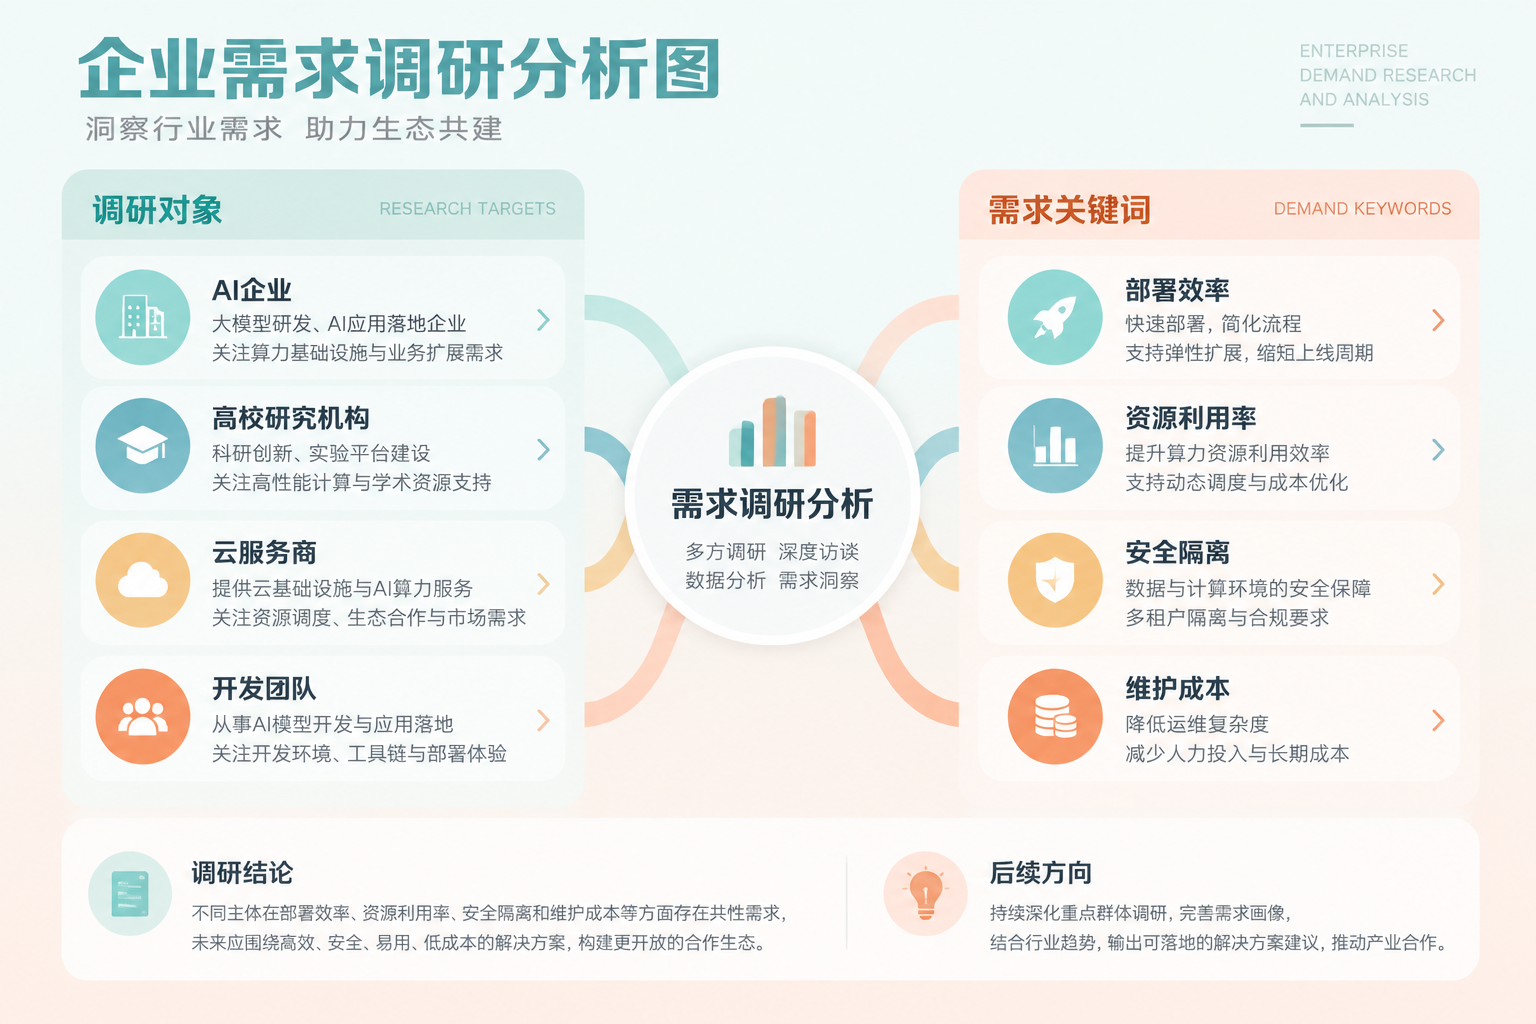
\includegraphics[width=\linewidth,height=.50\textheight,keepaspectratio]{figures/updated-4-1.png}
\caption{一手调研对象构成与需求分布图}\label{fig:4-1}
\par\vspace{3pt}{\fontsize{9}{12}\selectfont\linespread{1}\selectfont 注：本图仅概括调研对象类别与需求方向，不表示访谈频次或统计比例；访谈数量、身份和量化信息以表 4-7 及原始记录核实结果为准。}
\end{figure}
\subsection{企业需求与 PI OS 响应映射}\label{sec:4.6.3}
表 4-8 把访谈反映的客户痛点、对应的技术机制、当前可提供的证据和完成状态对应起来，说明调研结论如何落到项目工作中。

\FloatBarrier
\begingroup\linespread{1}\selectfont
\setcounter{table}{7}
\begin{longtable}{@{}>{\raggedright\arraybackslash}p{\dimexpr 0.18446\linewidth-1.4757\tabcolsep\relax}>{\raggedright\arraybackslash}p{\dimexpr 0.23872\linewidth-1.9097\tabcolsep\relax}>{\raggedright\arraybackslash}p{\dimexpr 0.23872\linewidth-1.9097\tabcolsep\relax}>{\raggedright\arraybackslash}p{\dimexpr 0.20616\linewidth-1.6493\tabcolsep\relax}>{\raggedright\arraybackslash}p{\dimexpr 0.13194\linewidth-1.0556\tabcolsep\relax}@{}}
\caption{企业需求、痛点与 PI OS 响应映射表}\label{tab:4-8}\\
\hline
\rowcolor{WordTableHeader} \TableHeaderText{客户群体} & \TableHeaderText{访谈反映的核心痛点} & \TableHeaderText{对应技术机制} & \TableHeaderText{当前可提供的证据} & \TableHeaderText{状态} \\ \hline
\endfirsthead
\multicolumn{5}{c}{\fontsize{9}{12}\selectfont 表 4-8（续）}\\
\hline
\rowcolor{WordTableHeader} \TableHeaderText{客户群体} & \TableHeaderText{访谈反映的核心痛点} & \TableHeaderText{对应技术机制} & \TableHeaderText{当前可提供的证据} & \TableHeaderText{状态} \\ \hline
\endhead
\hline\endfoot\hline\endlastfoot
\rowcolor{WordTableStripe} 
AI 编程平台、智能体应用开发企业 & 高峰并发受限、任务排队、扩容成本高 & 运行时扁平化降低单实例固定开销；动态资源卸载回收等待阶段的驻留资源 & 表 3-1 卸载开销对比、表 3-2 受限资源下的系统级对比 & 研究环境已实测，待华为指定环境复测 \\ \hline
企业内部研发中心（研发管理） & 服务器资源紧张、环境维护工作量大 & 运行时扁平化减少重复部署；部署工具与文档降低维护负担 & 系统设计材料（V-02）、部署流程草案 & 方案已形成，部署工具正在完善 \\ \hline
\rowcolor{WordTableStripe} 
企业内部研发中心（信息化与安全） & 数据不出内网、多租户隔离与审计要求 & 共享边界由内容、版本、访问权限和状态可变性共同确定，私有状态保留独立副本 & 第 3.6 节共享边界说明、表 7-2 风险与对策映射 & 机制已设计，需在指定环境完成隔离测试 \\ \hline
高校实验室、研究所及模型评测团队 & 环境重复配置、批量任务难以复现 & 智能内存共享消除跨实例重复状态；脚本与复现说明保证一致性 & 图 3-8、S-01---S-06 复现说明 & 研究环境已验证，可提供试用 \\ \hline
\rowcolor{WordTableStripe} 
云服务商、系统集成商 & 自研投入大、适配与交付成本高 & 提供运行引擎集成、环境适配与维护支持 & 第 4.4 节商业模式、交付流程草案 & 待产品标准化后拓展 \\ \hline
\end{longtable}\endgroup
图 4-2 以映射关系的方式呈现“客户需求---技术机制---证据材料”的对应，说明调研结论已在技术工作中得到响应。

\begin{figure}[H]\centering
\setcounter{figure}{1}
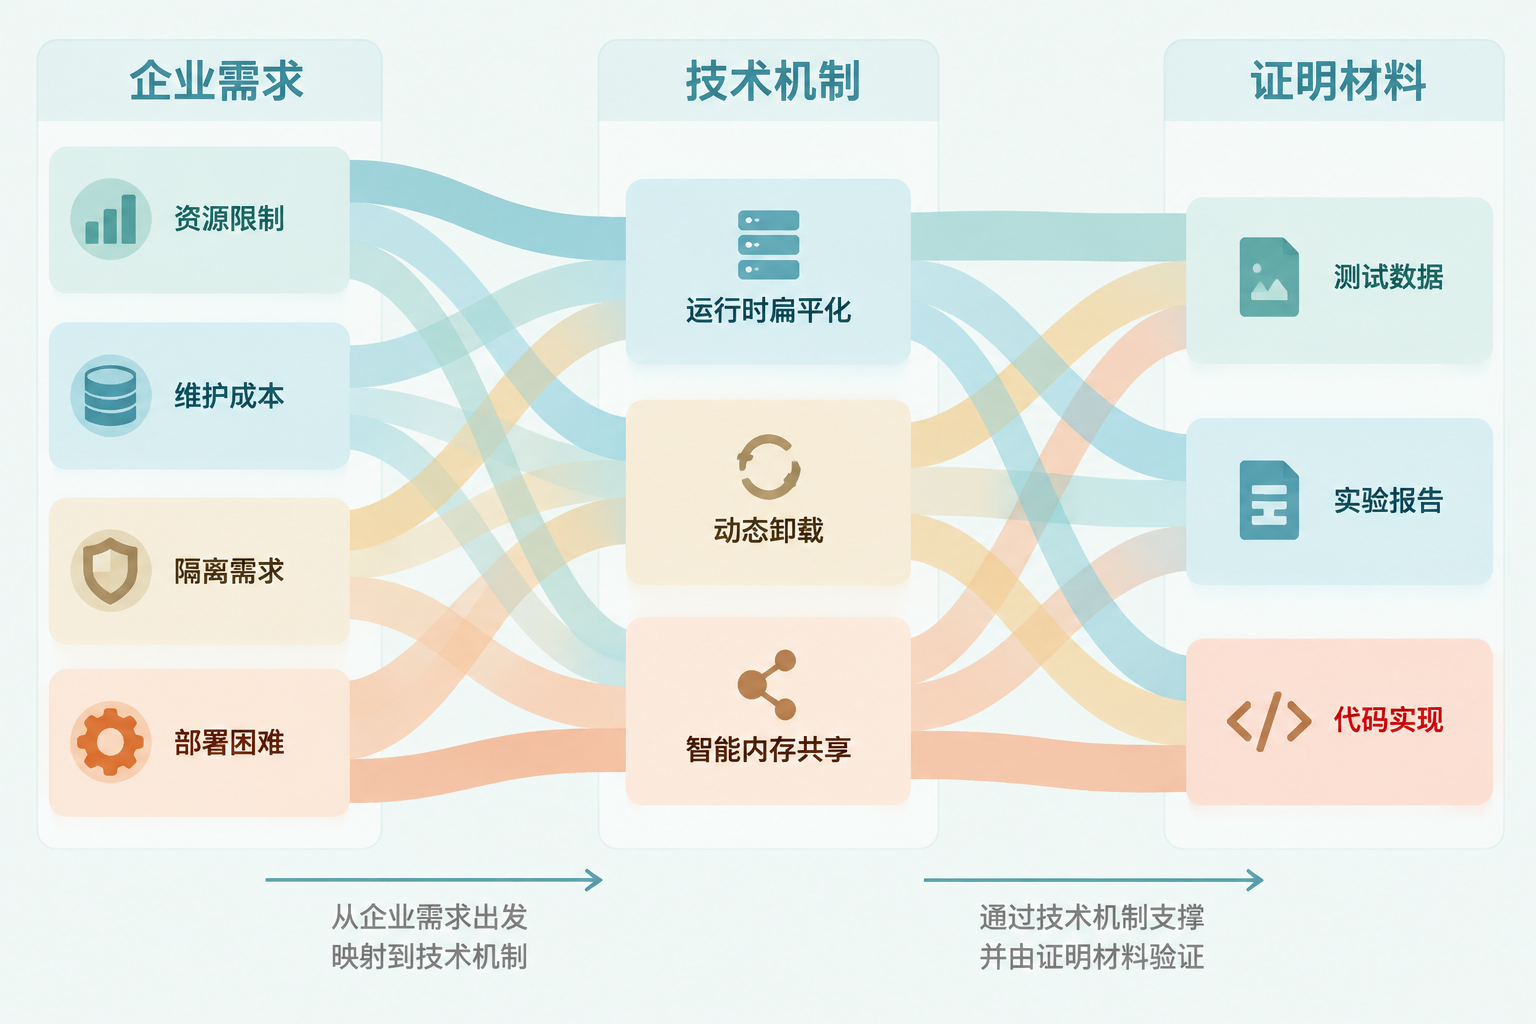
\includegraphics[width=\linewidth,height=.50\textheight,keepaspectratio]{figures/updated-4-2.png}
\caption{企业需求、技术机制与证据材料映射图}\label{fig:4-2}
\par\vspace{3pt}{\fontsize{9}{12}\selectfont\linespread{1}\selectfont 注：连线仅表示需求与机制的示意联系，不表示已完成验证或覆盖程度；机制状态与证据范围以表 4-8 为准。}
\end{figure}
\subsection{采购流程、部署周期与价格接受范围}\label{sec:4.6.4}
调研显示，企业采购智能体运行环境通常需要经过四个环节：技术验证、内部试点、预算审批和正式采购。技术验证阶段由技术负责人主导，关注功能与性能是否达到要求；内部试点阶段由使用部门主导，关注真实任务中的稳定性与效率；预算审批阶段由信息化或财务部门参与，关注投入规模、付款方式和合规要求；正式采购阶段涉及合同、交付与验收条款。四个环节的推进周期受企业规模与合规要求影响，是项目安排销售节奏与现金流测算的重要依据。

\FloatBarrier
\begingroup\linespread{1}\selectfont
\setcounter{table}{8}
\begin{longtable}{@{}>{\raggedright\arraybackslash}p{\dimexpr 0.15191\linewidth-1.2153\tabcolsep\relax}>{\raggedright\arraybackslash}p{\dimexpr 0.21701\linewidth-1.7361\tabcolsep\relax}>{\raggedright\arraybackslash}p{\dimexpr 0.23872\linewidth-1.9097\tabcolsep\relax}>{\raggedright\arraybackslash}p{\dimexpr 0.15734\linewidth-1.2587\tabcolsep\relax}>{\raggedright\arraybackslash}p{\dimexpr 0.23503\linewidth-1.8802\tabcolsep\relax}@{}}
\caption{企业采购决策链、部署周期与项目可提供的工作}\label{tab:4-9}\\
\hline
\rowcolor{WordTableHeader} \TableHeaderText{环节} & \TableHeaderText{主导角色} & \TableHeaderText{判断依据} & \TableHeaderText{典型周期} & \TableHeaderText{学生团队可提供的工作} \\ \hline
\endfirsthead
\multicolumn{5}{c}{\fontsize{9}{12}\selectfont 表 4-9（续）}\\
\hline
\rowcolor{WordTableHeader} \TableHeaderText{环节} & \TableHeaderText{主导角色} & \TableHeaderText{判断依据} & \TableHeaderText{典型周期} & \TableHeaderText{学生团队可提供的工作} \\ \hline
\endhead
\hline\endfoot\hline\endlastfoot
\rowcolor{WordTableStripe} 
技术验证 & 技术负责人、研发平台负责人 & 功能可用性、并发能力、任务成功率 & 2---4 周（待填实测值） & 提供演示环境与对照测试方案，配合客户完成同一批任务的对比测试 \\ \hline
内部试点 & 使用部门负责人 & 真实任务中的稳定性、效率改善、维护负担 & 1---3 个月 & 提供部署指南与使用文档，配合现场支持，整理试点期间的任务与资源数据 \\ \hline
\rowcolor{WordTableStripe} 
预算审批 & 信息化部门、财务部门 & 投入规模、付款方式、合规与授权边界 & 1---2 个月 & 提供成果权属与授权范围说明、分档报价方案与分期服务方案 \\ \hline
正式采购与交付 & 采购部门、管理部门 & 合同条款、交付验收标准、售后责任 & 1---2 个月 & 签订交付与维护条款，完成部署、使用培训与验收 \\ \hline
\end{longtable}\endgroup
关于价格接受范围，受访对象未给出统一区间，但提供了三类判断线索：一是与“新增一台服务器”的成本比较，若方案能够在现有服务器上承载更多任务，客户愿意以低于扩容成本的金额采购；二是与“按并发计费的商业沙箱服务”比较，客户关注计费是否与实际消耗一致，倾向于为实际节省的资源付费；三是与服务能力挂钩，包含部署适配、维护与响应的服务方案更容易被接受。据此，项目将价格锚定在客户可核算的资源节省上，并在第 4.4.5 节给出分档收费的初步设计，具体报价在试点阶段结合真实任务量与资源数据确定。

\par\noindent{\fontsize{9}{13}\selectfont\linespread{1}\selectfont 注：本节采购周期与价格信息为访谈中的定性描述，不代表已确认的商务条件；正式报价与合同条款以双方签署文件为准。表 4-9 中的典型周期应在完成首批试点后以实测数据替换。}

图 4-3 呈现采购决策链中各环节的推进关系与项目介入点。

\begin{figure}[H]\centering
\setcounter{figure}{2}
\begin{tikzpicture}[x=1cm,y=1cm, every node/.style={font=\fontsize{9}{12}\selectfont\linespread{1}\selectfont,align=center},box/.style={draw=DiagramRule,rounded corners=2pt,fill=DiagramLight,inner sep=6pt},arr/.style={->,>=stealth,thick,draw=DiagramMain}]
\node[box,text width=2.7cm,] (stage0) at (1.6,0.0) {\textbf{技术验证}\\2---4 周（待填实测值）};
\node[box,text width=3cm,] (owner0) at (5,0.0) {技术负责人、研发平台负责人\\功能可用性、并发能力、任务成功率};
\node[box,text width=5.8cm,fill=DiagramMedium] (work0) at (10,0.0) {提供演示环境与对照测试方案，配合客户完成同一批任务的对比测试};
\draw[arr] (stage0) -- (owner0);\draw[arr] (owner0) -- (work0);
\node[box,text width=2.7cm,] (stage1) at (1.6,-2.1) {\textbf{内部试点}\\1---3 个月};
\node[box,text width=3cm,] (owner1) at (5,-2.1) {使用部门负责人\\真实任务中的稳定性、效率改善、维护负担};
\node[box,text width=5.8cm,fill=DiagramMedium] (work1) at (10,-2.1) {提供部署指南与使用文档，配合现场支持，整理试点期间的任务与资源数据};
\draw[arr] (stage1) -- (owner1);\draw[arr] (owner1) -- (work1);
\draw[arr] (stage0) -- (stage1);
\node[box,text width=2.7cm,] (stage2) at (1.6,-4.2) {\textbf{预算审批}\\1---2 个月};
\node[box,text width=3cm,] (owner2) at (5,-4.2) {信息化部门、财务部门\\投入规模、付款方式、合规与授权边界};
\node[box,text width=5.8cm,fill=DiagramMedium] (work2) at (10,-4.2) {提供成果权属与授权范围说明、分档报价方案与分期服务方案};
\draw[arr] (stage2) -- (owner2);\draw[arr] (owner2) -- (work2);
\draw[arr] (stage1) -- (stage2);
\node[box,text width=2.7cm,] (stage3) at (1.6,-6.300000000000001) {\textbf{正式采购与交付}\\1---2 个月};
\node[box,text width=3cm,] (owner3) at (5,-6.300000000000001) {采购部门、管理部门\\合同条款、交付验收标准、售后责任};
\node[box,text width=5.8cm,fill=DiagramMedium] (work3) at (10,-6.300000000000001) {签订交付与维护条款，完成部署、使用培训与验收};
\draw[arr] (stage3) -- (owner3);\draw[arr] (owner3) -- (work3);
\draw[arr] (stage2) -- (stage3);
\node[box,text width=12cm,] (note) at (6.5,-8) {周期来自阶段调研描述，须以试点实测更新；各阶段满足条件后再推进，不作为承诺工期。};
\end{tikzpicture}
\caption{企业采购决策链、部署周期与项目介入点图}\label{fig:4-3}
\end{figure}
\subsection{调研结论与市场进入策略修正}\label{sec:4.6.5}
依据调研结果，项目对市场进入策略作以下修正。

\NumberedPara{1}{首阶段客户聚焦两类：以代码修复、功能开发、自动测试为主要任务的 AI 编程平台，以及拥有内部研发智能体并使用自有服务器的企业内部研发中心。这两类客户任务边界清晰、资源压力可量化，便于在较短时间内形成可复核的效果对比。}
\NumberedPara{2}{定位表述从“提高部署密度”调整为“在同等硬件条件下提高可完成的任务数量”。前者是技术指标，后者是客户可直接感知的经营指标，也便于与客户的现有账本对照。}
\NumberedPara{3}{把“部署适配与维护服务”提前到首批交付内容中，而非留到产品成熟后再提供。调研显示适配成本是客户决策的实际门槛，提前提供该能力有助于缩短从技术验证到试点的周期。}
\NumberedPara{4}{对合规要求较高的客户，优先提供私有化部署方案与隔离机制说明，并准备多租户隔离与审计能力的验证材料，避免在验证尚不充分时同时铺开金融、工业等行业场景。}
上述修正已体现在第四章的目标市场（第 4.3 节）与商业模式（第 4.4 节）中。后续调研将围绕首批两类客户继续开展，重点补充真实任务量、资源使用数据与决策链信息，并将新增访谈记录纳入 I-xx 编号序列统一归档。

